\hypertarget{button_8hpp}{
\section{/home/arnaud/programmation/sfml/sfgui/button.hpp File Reference}
\label{button_8hpp}\index{/home/arnaud/programmation/sfml/sfgui/button.hpp@{/home/arnaud/programmation/sfml/sfgui/button.hpp}}
}
{\tt \#include $<$SFML/Graphics.hpp$>$}\par
{\tt \#include \char`\"{}object.hpp\char`\"{}}\par
{\tt \#include \char`\"{}constantes.hpp\char`\"{}}\par
{\tt \#include \char`\"{}margin.hpp\char`\"{}}\par
{\tt \#include $<$string$>$}\par


Include dependency graph for button.hpp:\nopagebreak
\begin{figure}[H]
\begin{center}
\leavevmode
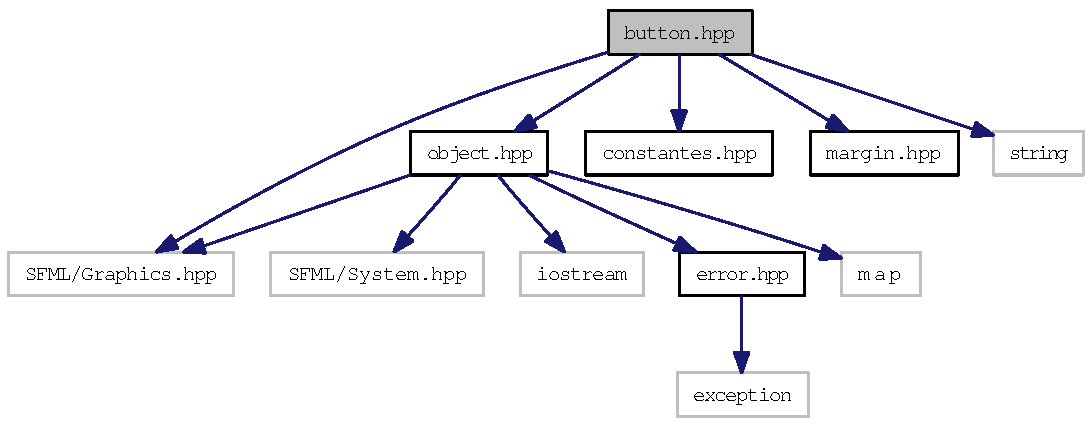
\includegraphics[width=279pt]{button_8hpp__incl}
\end{center}
\end{figure}


This graph shows which files directly or indirectly include this file:\nopagebreak
\begin{figure}[H]
\begin{center}
\leavevmode
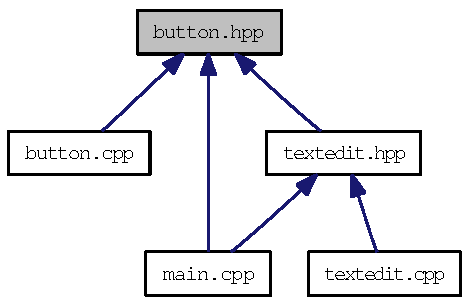
\includegraphics[width=376pt]{button_8hpp__dep__incl}
\end{center}
\end{figure}
\subsection*{Namespaces}
\begin{CompactItemize}
\item 
namespace \hyperlink{namespacesfgui}{sfgui}
\end{CompactItemize}
\subsection*{Classes}
\begin{CompactItemize}
\item 
class \hyperlink{classsfgui_1_1Button}{sfgui::Button}
\begin{CompactList}\small\item\em A push button. \item\end{CompactList}\end{CompactItemize}
